\documentclass[10pt, compress]{beamer}

\usetheme{metropolis}

\usepackage{booktabs}
\usepackage[scale=2]{ccicons}

\usepackage{amsmath}

%Icons
\usepackage{fontawesome}

%Syntax highlight
\usepackage{listings,xcolor}
\usepackage{inconsolata}

\definecolor{dkgreen}{rgb}{0,.6,0}
\definecolor{dkblue}{rgb}{0,0,.6}
\definecolor{dkyellow}{cmyk}{0,0,.8,.3}

% Language: PHP
\lstset{
  language        = php,
  basicstyle      = \small\ttfamily,
  keywordstyle    = \color{dkblue},
  stringstyle     = \color{red},
  identifierstyle = \color{dkgreen},
  commentstyle    = \color{gray},
  emph            =[1]{php},
  emphstyle       =[1]\color{black},
  emph            =[2]{if,and,or,else},
  emphstyle       =[2]\color{dkyellow}
}

%\usepgfplotslibrary{dateplot}


\title{Fun with symbolic execution}	
\subtitle{Exploit development and deobfuscation}
\date{\today}
\author{Carl Svensson}
\institute{SEC-T 2018}

\begin{document}

\maketitle

\begin{frame}{About me}
  
	\begin{columns}
		\begin{column}{0.6\textwidth}  
  
  		\begin{itemize}
		  \item Carl Svensson, 27
		  \item MSc in Computer Science, KTH
		  \item Head of Security, Kry
		  \item CTF-player, HackingForSoju
		  \item \faEnvelope \hskip 2mm calle.svensson@zeta-two.com
		  \item \faTwitter \hskip 2mm  @zetatwo
		  \item \faGlobe \hskip 2mm https://zeta-two.com
		\end{itemize}
		
		\end{column}
		\begin{column}{0.4\textwidth} 
			\begin{center}
			
\includegraphics[width=0.4\textwidth]{images/kth.jpg}
			\end{center}
			\vspace{1cm}
			
\includegraphics[width=\textwidth]{images/kry_logo.png}
		\end{column}
	\end{columns}
  
\end{frame}

\begin{frame}{Symbolic execution}
  \begin{itemize}
    \item Symbols vs. concrete values
    \item Pro: Explore "all" paths
    \item Con: Exponential complexity
  \end{itemize}
\end{frame}

\begin{frame}{Once again, with fee... angr}

  \begin{columns}
    \begin{column}{0.75\textwidth}
  
    \begin{itemize}
    \item "python framework for analyzing binaries"
    \item "both static and dynamic symbolic (concolic)"
    \item Computer Security Lab at UC Santa Barbara
    \item Uses Z3 internally
    \end{itemize}
  \end{column}
    \begin{column}{0.25\textwidth}
      
\includegraphics[width=\textwidth]{images/angr-logo.png}
    \end{column}
  \end{columns} 

\end{frame}

\begin{frame}{Exploitation}
  \begin{itemize}
    \item IP control
    \item Satisfy condition
  \end{itemize}
\end{frame}

\begin{frame}{Exploitation with angr}
  \begin{itemize}
    \item Find execution path
    \item Constrain execution
    \item Satisfy condition
  \end{itemize}
\end{frame}

\begin{frame}{Example from Security Fest CTF}
  \begin{itemize}
    \item Function pointer lookup
    \item Index OOB
    \item Hook messy function
  \end{itemize}
\end{frame}


\begin{frame}{angr exploitation example}
  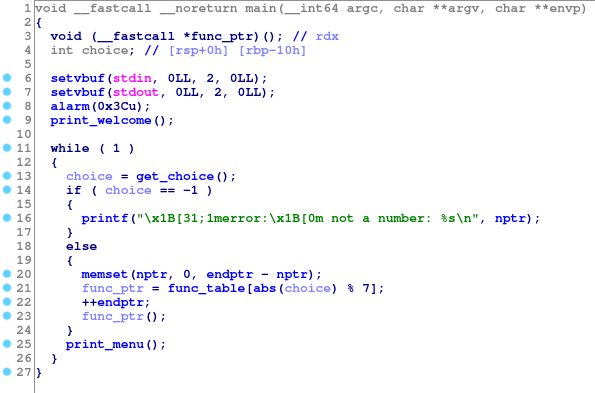
\includegraphics[width=0.8\textwidth]{images/exploit-2-ida.png}
\end{frame}

\begin{frame}{angr exploitation example}
  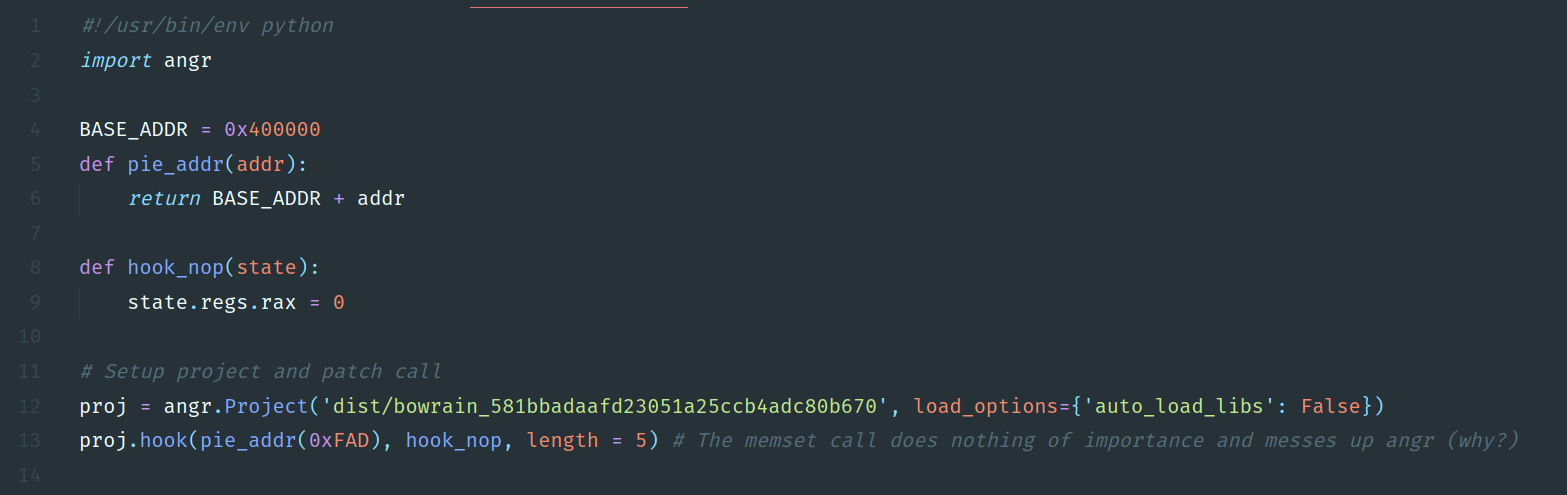
\includegraphics[width=\textwidth]{images/exploit-1-angr-a.png}
\end{frame}

\begin{frame}{angr exploitation example}
  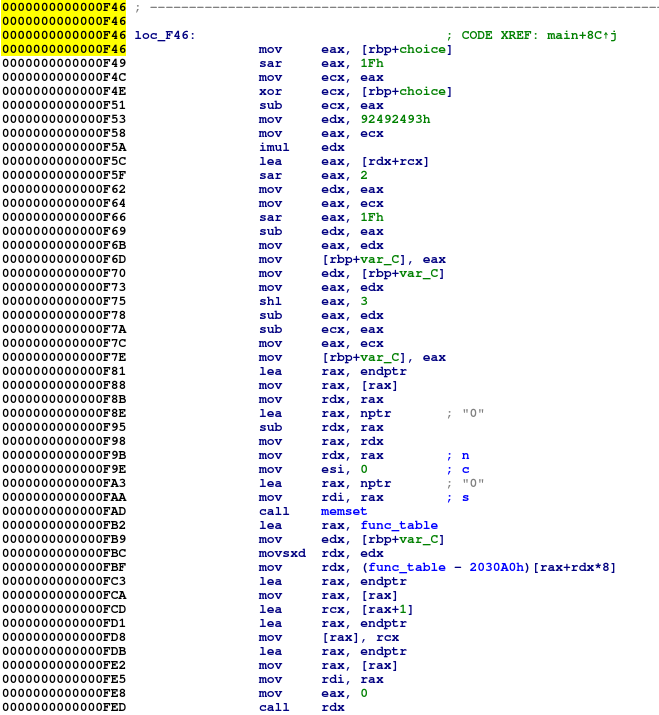
\includegraphics[width=0.5\textwidth]{images/exploit-2-ida2.png}
\end{frame}

\begin{frame}{angr exploitation example}
  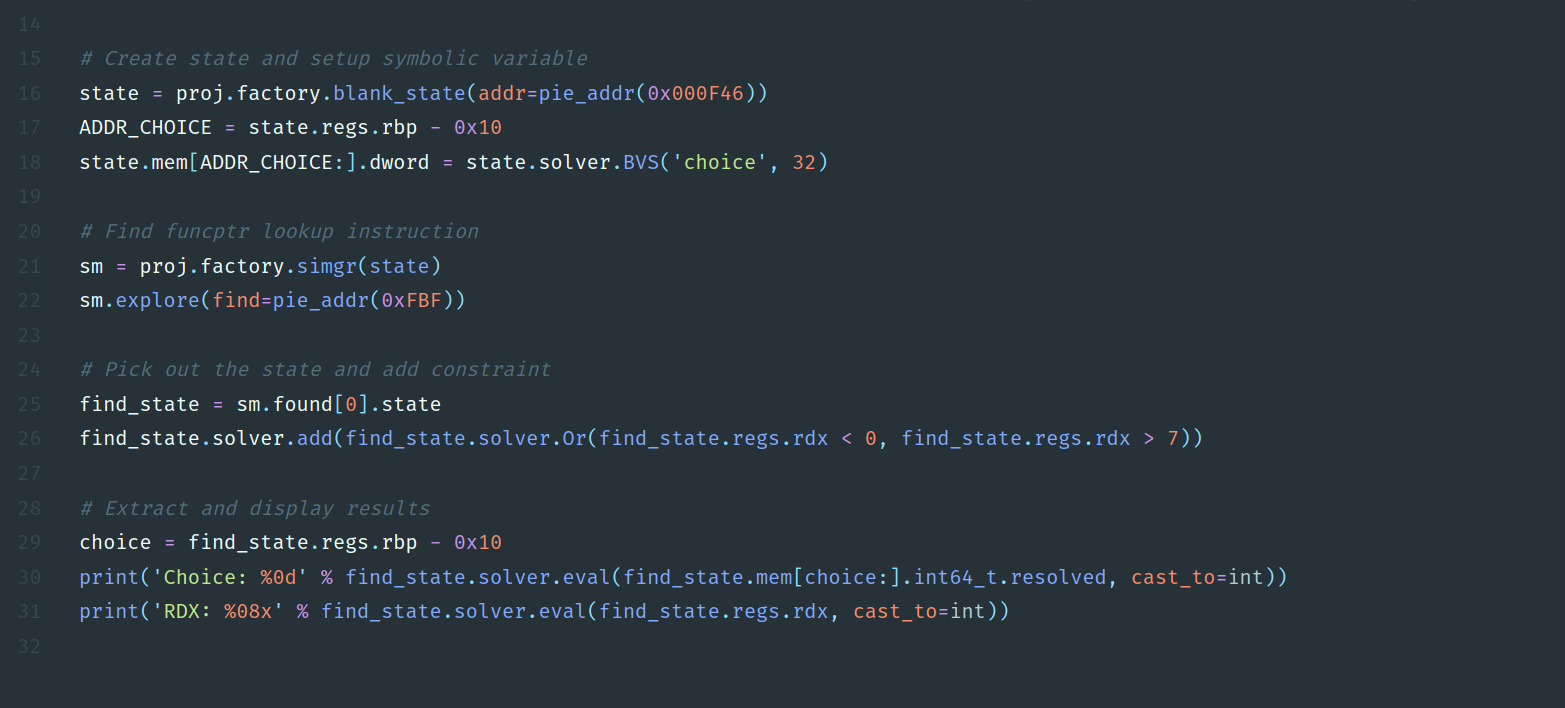
\includegraphics[width=\textwidth]{images/exploit-1-angr-b.png}
\end{frame}

\begin{frame}[fragile]{angr exploitation example}

\begin{lstlisting}[language=bash]
> python exploit_angr.py
Choice: 2147483648
RDX: fffffffffffffffe
\end{lstlisting}

\begin{lstlisting}[language=bash]
> ./bowrain_581bbadaafd23051a25ccb4adc80b670
...
: 2147483648
[1] 17059 segmentation fault (core dumped)
\end{lstlisting}

\end{frame}


\begin{frame}{Deobfuscation}
\section{Deobfuscation}
\end{frame}

\begin{frame}{Obfuscation}
  \begin{itemize}
    \item Make code hard to read
    \begin{itemize}
      \item for humans
      \item for computers
    \end{itemize}
    \item Control flow flattening
    \item Packer
    \item Dropper
    \item VM
    \item Dead code
  \end{itemize}
\end{frame}

\begin{frame}{Deobfuscation in general}
  \begin{itemize}
    \item Undo the mess
    \item Hard problem
  \end{itemize}
\end{frame}

\begin{frame}{Deobfuscation of dead code with angr}
  \begin{itemize}
    \item Prove that dead code is dead
    \item Prove uniqueness of value
  \end{itemize}
\end{frame}

\begin{frame}{Example: indirect jmp deobfuscator}
\begin{center}
  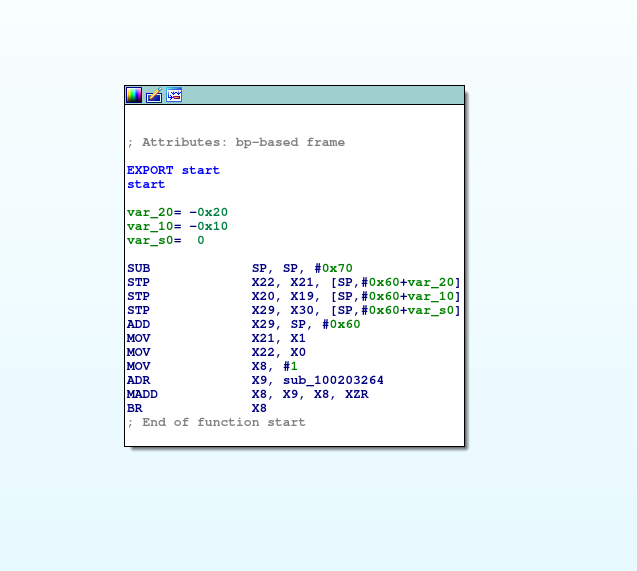
\includegraphics[width=0.6\textwidth]{images/deobf-1-ida1.png}
 \end{center}
\end{frame}

\begin{frame}{Example from mobile app}
  \begin{itemize}
    \item Find "jmp reg"
    \item Search callgraph backwards
    \item Search forward
    \item Simplify expression
    \item Replace code
  \end{itemize}
\end{frame}

\begin{frame}{Example: indirect jmp deobfuscator}
\begin{center}
  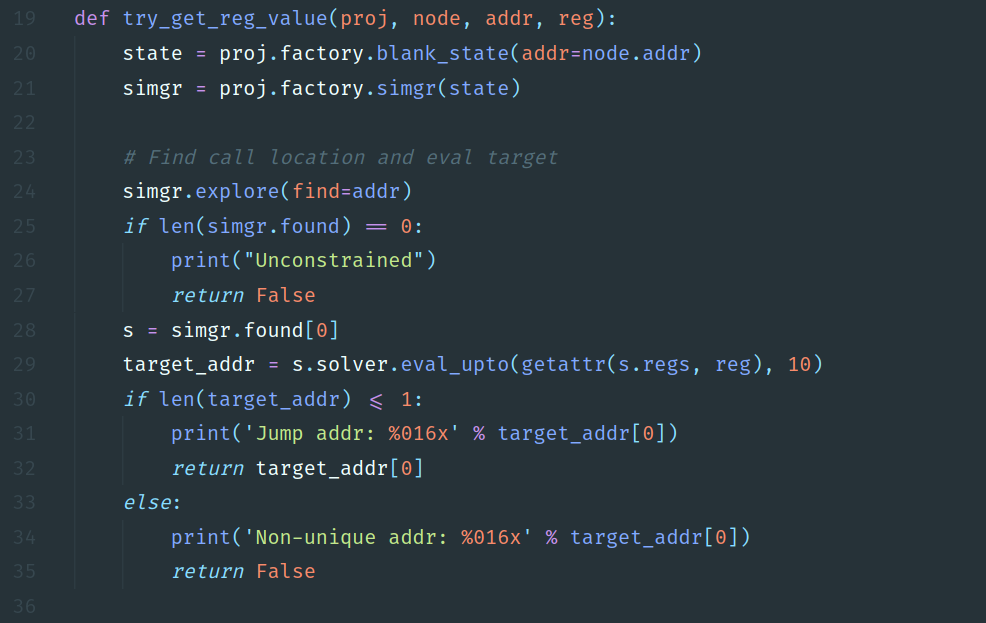
\includegraphics[width=0.8\textwidth]{images/deobf-4-angr1.png}
 \end{center}
\end{frame}

\begin{frame}{Example: indirect jmp deobfuscator}
\begin{center}
  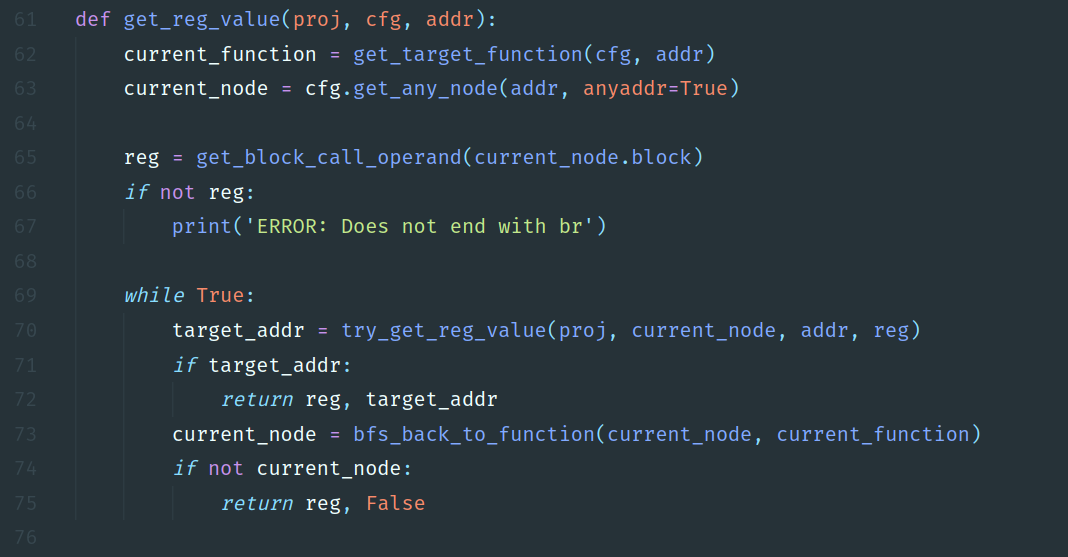
\includegraphics[width=0.8\textwidth]{images/deobf-5-angr2.png}
 \end{center}
\end{frame}


\begin{frame}{Example: indirect jmp deobfuscator}
\begin{center}
  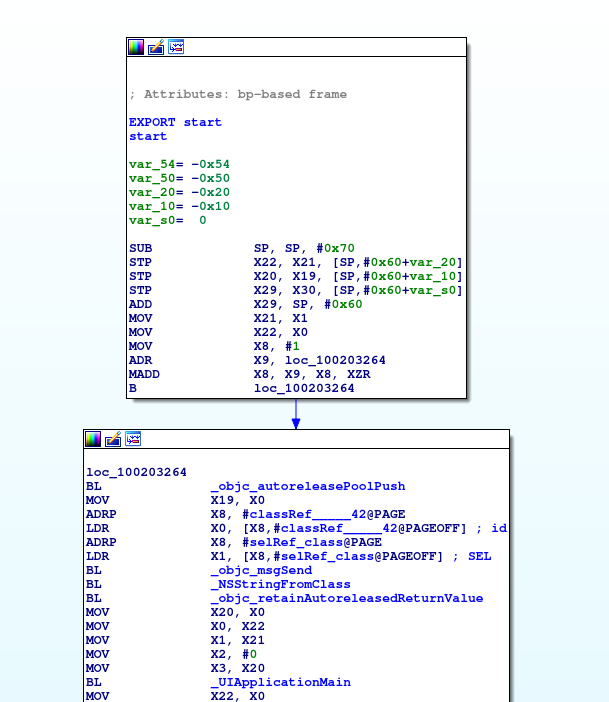
\includegraphics[width=0.5\textwidth]{images/deobf-2-ida2.png}
   \end{center}
\end{frame}

\begin{frame}{Example: indirect jmp deobfuscator}
\begin{center}
  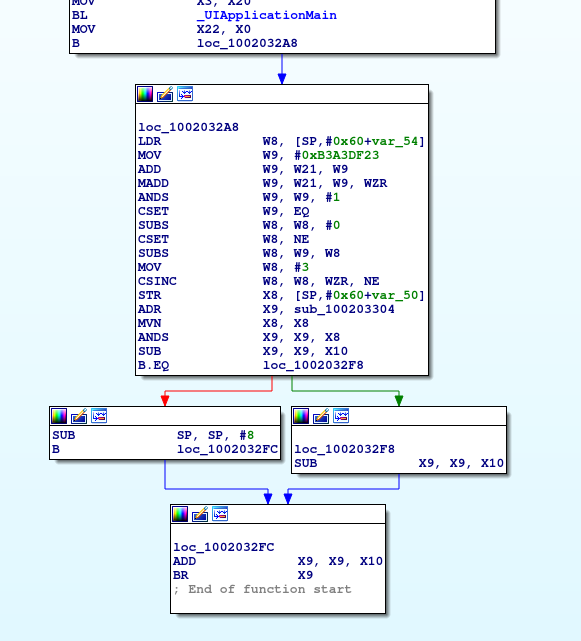
\includegraphics[width=0.5\textwidth]{images/deobf-3-ida3.png}
   \end{center}
\end{frame}

\begin{frame}[standout]
Thanks for listening!
\end{frame}

\end{document}
